% THIS IS SIGPROC-SP.TEX - VERSION 3.1
% WORKS WITH V3.2SP OF ACM_PROC_ARTICLE-SP.CLS
% APRIL 2009
%
% It is an example file showing how to use the 'acm_proc_article-sp.cls' V3.2SP
% LaTeX2e document class file for Conference Proceedings submissions.
% ----------------------------------------------------------------------------------------------------------------
% This .tex file (and associated .cls V3.2SP) *DOES NOT* produce:
%       1) The Permission Statement
%       2) The Conference (location) Info information
%       3) The Copyright Line with ACM data
%       4) Page numbering
% ---------------------------------------------------------------------------------------------------------------
% It is an example which *does* use the .bib file (from which the .bbl file
% is produced).
% REMEMBER HOWEVER: After having produced the .bbl file,
% and prior to final submission,
% you need to 'insert'  your .bbl file into your source .tex file so as to provide
% ONE 'self-contained' source file.
%
% Questions regarding SIGS should be sent to
% Adrienne Griscti ---> griscti@acm.org
%
% Questions/suggestions regarding the guidelines, .tex and .cls files, etc. to
% Gerald Murray ---> murray@hq.acm.org
%
% For tracking purposes - this is V3.1SP - APRIL 2009

\documentclass{acm_proc_article-sp}

\begin{document}
\title{Energy Based Location Prediction}

\numberofauthors{4}
\author{
% 1st. author
\alignauthor
Gayatri Sivaraman
\email{gayatri267@utexas.edu}
% 2nd. author
\alignauthor
Jayant Bedwal
\email{jayant21@utexas.edu}
% 3rd. author
\alignauthor
Shailesh Kelkar
\email{shaileshsk94@utexas.edu}
% use '\and' if you need 'another row' of author names
% 4th. author
\alignauthor
Srihari Venugopalan
\email{sriharivenu@utexas.edu}
\and
The University of Texas at Austin
}

\maketitle
\begin{abstract}
Location estimation is an important part of many ubiquitous computing systems. This report presents a research study to identify how well does inertial sensor data independently determine the location context of a person. A Wearable device was used to collect the inertial sensor data of people at different locations. None of the location specific data (like GPS, WiFi, Audio ) were collected. A methodology for preprocessing the data and extracting features for getting the best accuracy for the classification system is specified. Results produced by different classifiers have been compared and studied. Based on this study, it can be concluded that inertial sensing data has a good correlation to the location context and can be used to identify the surrounding location even in the absence of infrastructure mediated sensing data. This reduces the privacy based issues which persist in location context detection using infrastructure mediated sensors.
\end{abstract}

\keywords{Sensus Application, Inertial Sensing, FIR Filter, SVM, Random Forest, KNN, Split-Train Test Technique.} % NOT required for Proceedings

\section{Introduction}
Identifying a person\textsc{\char39}s current location and recognizing what he or she is doing \textsc{\char45} is a key functionality in many pervasive computing applications. Activity recognition using inertial sensing is a well-established research field with considerable amount of work being done to analyze sensor data to detect the activity. This research began with identifying the dependence between activity being performed and the location at which it is performed. If an inter\textsc{\char45}dependence exists, then the inertial sensing data could be exploited to train models which can identify the kind of place the person is currently located at. This research has produced promising results with the classifier working with an accuracy of 79\textsc{\char37}  
This new approach towards location identification can eliminate the privacy issues that occur when infrastructure mediated sensing devices are used to identify location context.

\section{Motivation}
Location sensing using inertial data has been a widely researched field. In several mobile computing studies\cite{Constandache:Bob}, sound beaconing has been employed to estimate relative positions to other devices. Kunze et al\cite{Kunze:Ubicomp}. proposed an absolute positioning method that estimates where a phone is placed combining vibration and short, narrow frequency beeps to sample the response of an environment. Rossi et al.\cite{Rossi:2013:RIP:2459236.2459252} proposed a positioning method using smartphones based on the background sounds. The authors measure impulse response at each indoor position and train a classifier that predicts a user\textsc{\char39}s current position using the observed impulse response. Tung et al.\cite{Tung:2015:EAI:2789168.2790102} employed an active sound probing for indoor location tagging and achieved 1 cm resolution. 
This research in contrast to the above mentioned work, was oriented towards using inertial data collected only from the user without using any infrastructure mediated sensing. Moreover, analysis was done, to find whether the activity being performed has a correlation to the location where it is being performed. If there does exist this correlation, then a prediction of the location context without collecting any location dependent data can be performed. This can considerably reduce privacy concerns related to using cameras or microphones to collect location dependent data. Also, this method can be used to differentiate between locations where the activities being performed are quite similar for eg. attending a lecture and reading at a library. 

\section{Contribution}
The contribution of the project:
\begin{itemize}
\item  New approach of determining location using inertial, heart rate and skin temperature sensors present in wearable devices.
\item Independent of any infrastructure mediated sensors which reduces privacy concerns.
\item Person independent approach for accurate location prediction.
\item Able to differentiate different locations having similar activities.
\end{itemize}

\section{Description}
\subsection{Data Collection}

\begin{enumerate}
\item \textbf{Device} :
Initially,a mobile phone was used for collecting inertial sensor data. An android application specific to the task was created, in order to extract accelerometer and gyroscope data from a smartphone. 8 participants volunteered for our study. From the analysis of the data collection process and the outcomes, it was observed that the phone data is not the true representative of energy pattern for a particular place. This is further supported by a research paper\cite{Dey:2011:GCE:2030112.2030135}.
The participants had their mobile phone either in a bag or pocket during the entire duration of the activity under consideration for example, in gym, the participants kept the mobile phone at a distant place like their locker. Hence, a Microsoft band was used for collection of data. The results (as shown in Fig ~\ref{fig:pic6}, Fig~\ref{fig:pic4} and Fig~\ref{fig:pic5}) were in favour of our analysis, so it was decided to go ahead with using the Microsoft Band for further data collection process.

\begin{figure}[h]
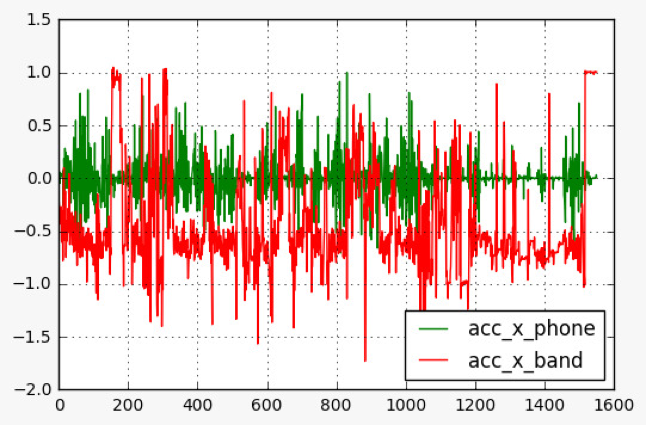
\includegraphics[scale=0.75]{Picture6.png}
\caption{Accelerometer X-axis readings for Phone vs Microsoft Band}
\label{fig:pic6}
\end{figure}

\begin{figure}[h]
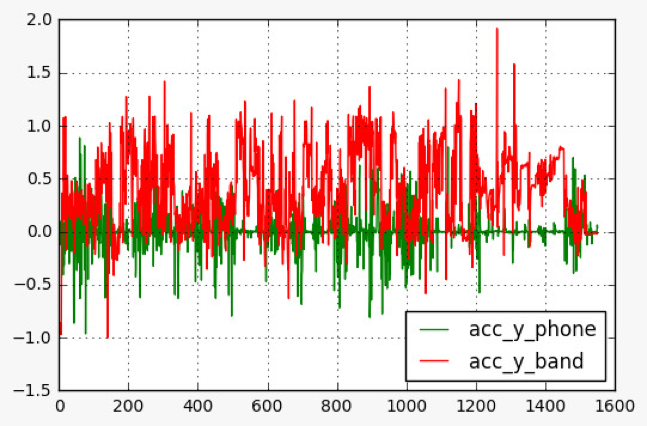
\includegraphics[scale=0.75]{Picture4.png}
\caption{Accelerometer Y-axis readings for Phone vs Microsoft Band}
\label{fig:pic4}
\end{figure}

\begin{figure}[h]
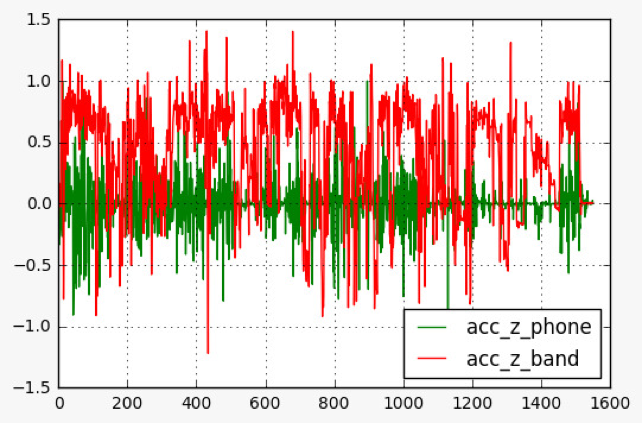
\includegraphics[scale=0.75]{Picture5.png}
\caption{Accelerometer Z-axis readings for Phone vs Microsoft Band}
\label{fig:pic5}
\end{figure}

\item \textbf{Sensus Application and AWS}  10 participants volunteered for the data collection process. The data was collected using Sensus\cite{Xiong:2016:SCG:2971648.2971711} Application on Android platform. The application was installed and a configuration file was provided to the participants by email which configured the application to probe smartphone and Microsoft band sensors as required for the research. The data collected by the application was directly uploaded to the AWS server at regular intervals of time. This ensured that there was no unnecessary build up of data on the user's smartphone.  

\item \textbf{Location Contexts}
 Locations targeted and the kind of activity performed there:
\begin{itemize}
\item Classroom: The volunteers were asked to wear the Microsoft band on the dominant hand and attend a 75 min lecture.
\item Library: 2 different activities were performed by the volunteers- Studying and stacking books. Both the activities were performed for 60 min duration.
\item Grocery Store: The volunteer used a shopping cart around the store and shopped for around 45 mins.
\item Recreation center/Gymnasium: The volunteer were asked to perform activities like weight training, treadmill, playing squash, racquetball etc. for around 60 min.
\end{itemize}
Sensors used to collect data were:
\begin{enumerate}
\item Accelerometer
\item Gyroscope
\item Skin Temperature
\item Heart Rate
\end{enumerate}

\subsection{Preprocessing}
The data collected was pre-processed by applying a variety of filters before choosing the apt one. By analyzing the techniques presented in \cite{Gjoreski11accelerometerdata}  ,the following filters were tried: FIR filter(Rectangular), Filt Filter, Median Filter, L Filter as shown in the Fig~\ref{fig:pic1} and Fig~\ref{fig:pic2}. It was decided to use FIR Filter for Gyroscope data and Median Filter for Accelerometer values. This decision was made after analyzing the accuracy of the Random forest classifier with 10 fold Cross Validation. The accuracy was 91\textsc{\char37} when median filter was used for both accelerometer and gyroscope data and 95\textsc{\char37} when median filter for accelerometer and FIR for gyroscope data were used. The performance of L filter and Filt filter was not as good as the other filters.

\begin{figure}[H]
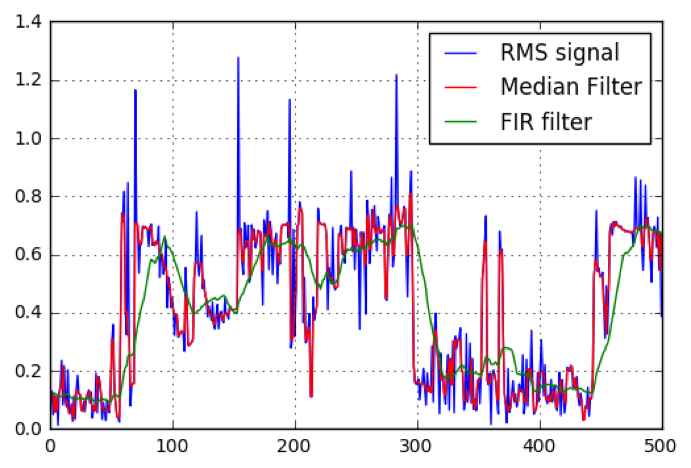
\includegraphics[scale=0.75]{Picture1.png}
\caption{Comparison of Median and FIR Filter for Accelerometer}
\label{fig:pic1}
\end{figure}

\begin{figure}[H]
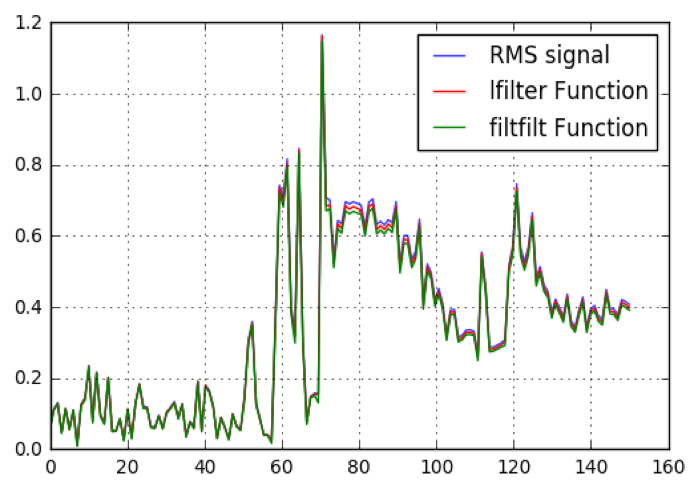
\includegraphics[scale=0.75]{Picture2.png}
\caption{Comparison of LFilter and FiltFilt Filter for Accelerometer}
\label{fig:pic2}
\end{figure}

\subsection{Frame extraction and Feature Selection}
Feature Extraction is an important parameter that helps in increasing the accuracy of the classifier. The work presented by Zhang et. al.  \cite{Zhang:2011:FSF:2318776.2318798} was used to get an idea about features of importance for the concerned problem.  
The following features were extracted from our dataset 
\begin{enumerate}
\item Mean (accelerometer, gyroscope, heart rate, skin temperature)
\item Variance (accelerometer, gyroscope)
\item RMS (accelerometer, gyroscope)
\item Mean and variance of RMS ( accelerometer only)
\end{enumerate}

\begin{table*}[p]
\centering
\caption{KNN Confusion Matrix Frame Size =105 Step Size =75}
\begin{tabular}{|c|c|c|c|c|l|} \hline
 &Library&grocery Store& Gym/Recreation center& Class & Library Stacking Books\\ \hline
\texttt{Library} & 0.40& 0.09& 0.05& 0.02& 0.74\\ \hline
\texttt{Grocery Store} & 0.05 & 0.79& 0.03& 0.01& 0.05\\ \hline
\texttt{Gym/Recreation Center}& 0.02& 0.01& 0.82& 0.00& 0.00\\ \hline
\texttt{Class}& 0.03& 0.03& 0.06& 0.94& 0.02\\ \hline
\texttt{Library Stacking Books}& 0.50& 0.06& 0.03& 0.02& 0.18\\ \hline
\end{tabular}
\label{table:tableKNN}
\end{table*}

\begin{table*}[p]
\centering
\caption{Random Forest Confusion Matrix Frame Size =90 Step Size =80}
\begin{tabular}{|c|c|c|c|c|l|} \hline
 &Library&grocery Store& Gym/Recreation center& Class & Library Stacking Books\\ \hline
\texttt{Library} & 0.65& 0.10& 0.02& 0.02& 0.03\\ \hline
\texttt{Grocery Store} & 0.08 & 0.85& 0.02& 0.01& 0.05\\ \hline
\texttt{Gym/Recreation Center}& 0.01& 0.01& 0.88& 0.02& 0.03\\ \hline
\texttt{Class}& 0.01& 0.03& 0.05& 0.92& 0.02\\ \hline
\texttt{Library Stacking Books}& 0.25& 0.02& 0.03& 0.03& 0.58\\ \hline
\end{tabular}
\label{table:tableRF}
\end{table*}




\subsection{Training the classifier}
To extract features from the collected data, a range of frame size and step size was chosen. The frame size varied from 50 to 200, in increments of 5 and the Step Size varied between 25 to 100, also in increments of 5.
\\

\begin{figure*}[p]
\centering
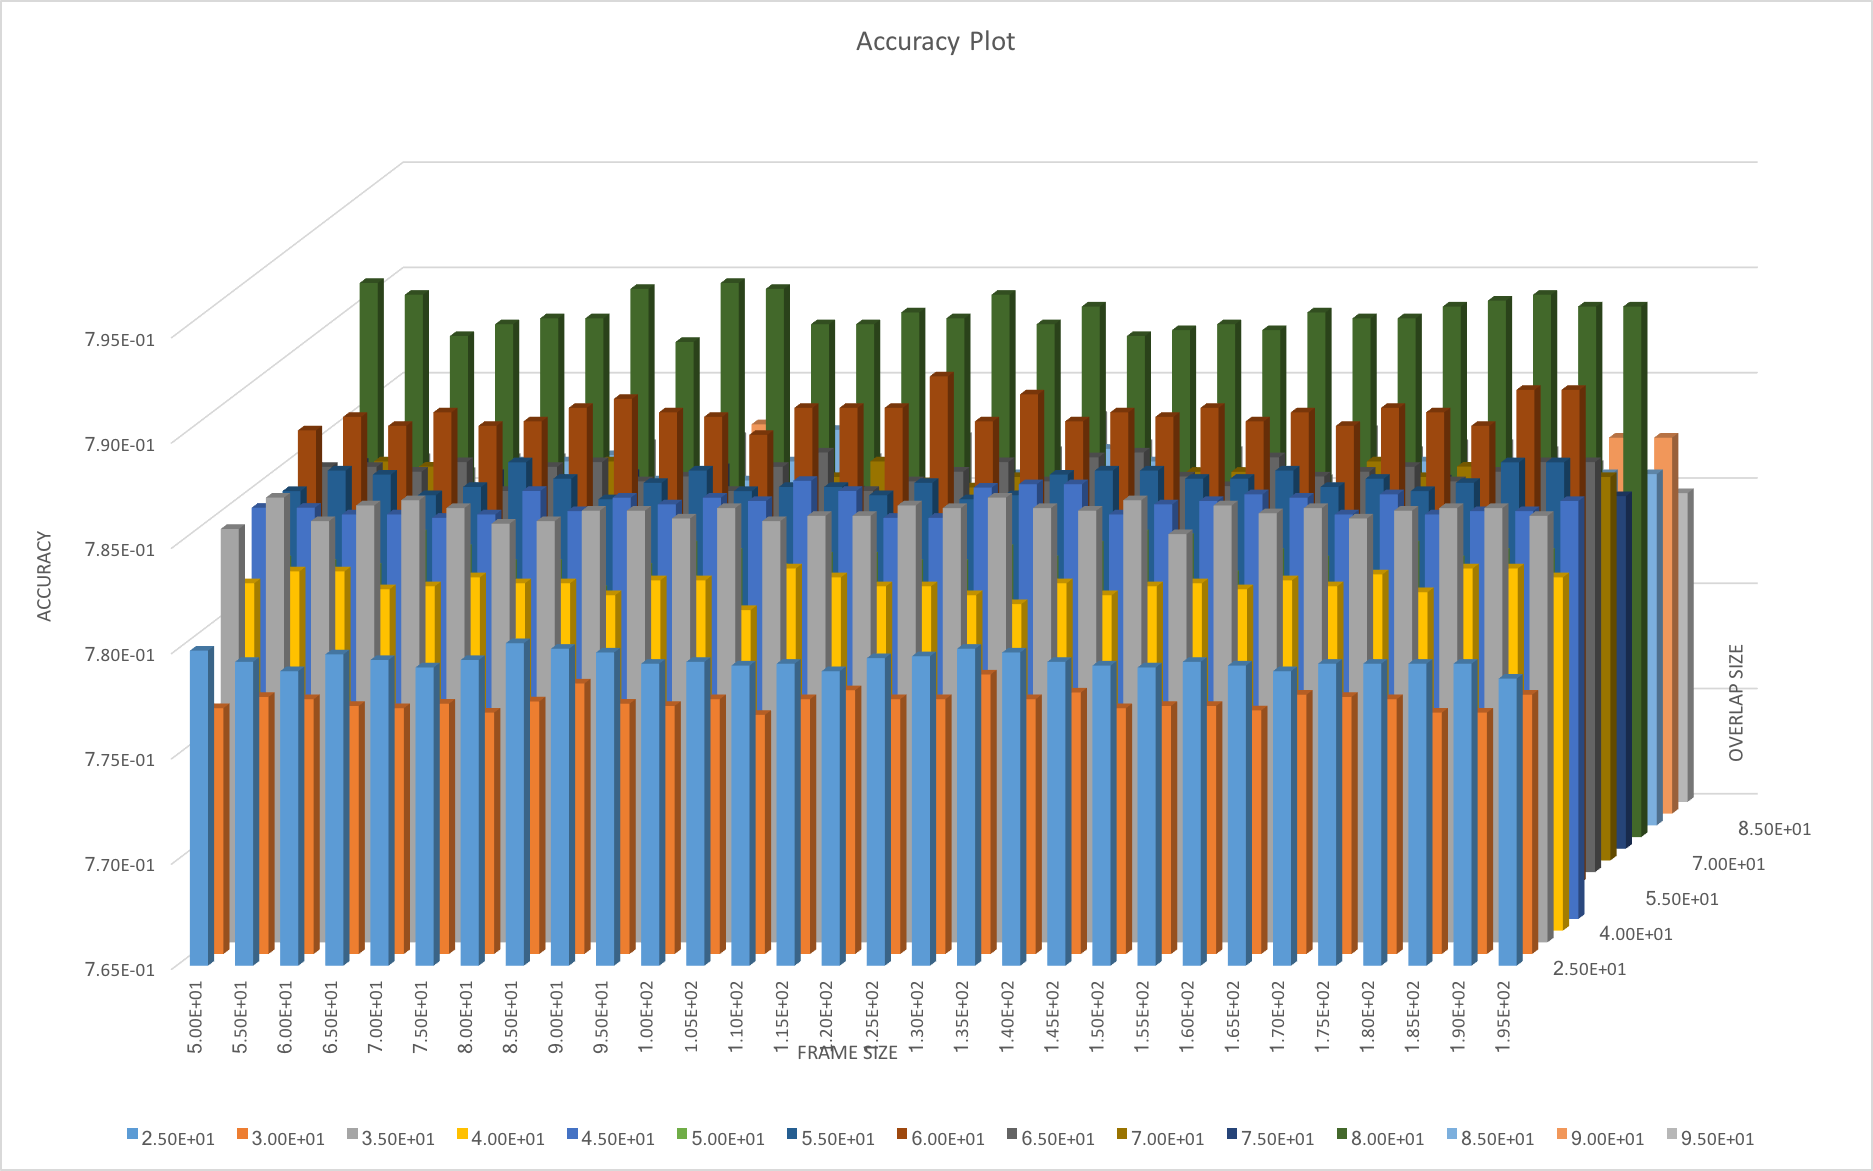
\includegraphics[scale=0.30]{PictureRF.png}
\caption{Accuracy plot for Random Forest}
\label{fig:picRF}
\end{figure*}

\begin{figure*}[p]
\centering
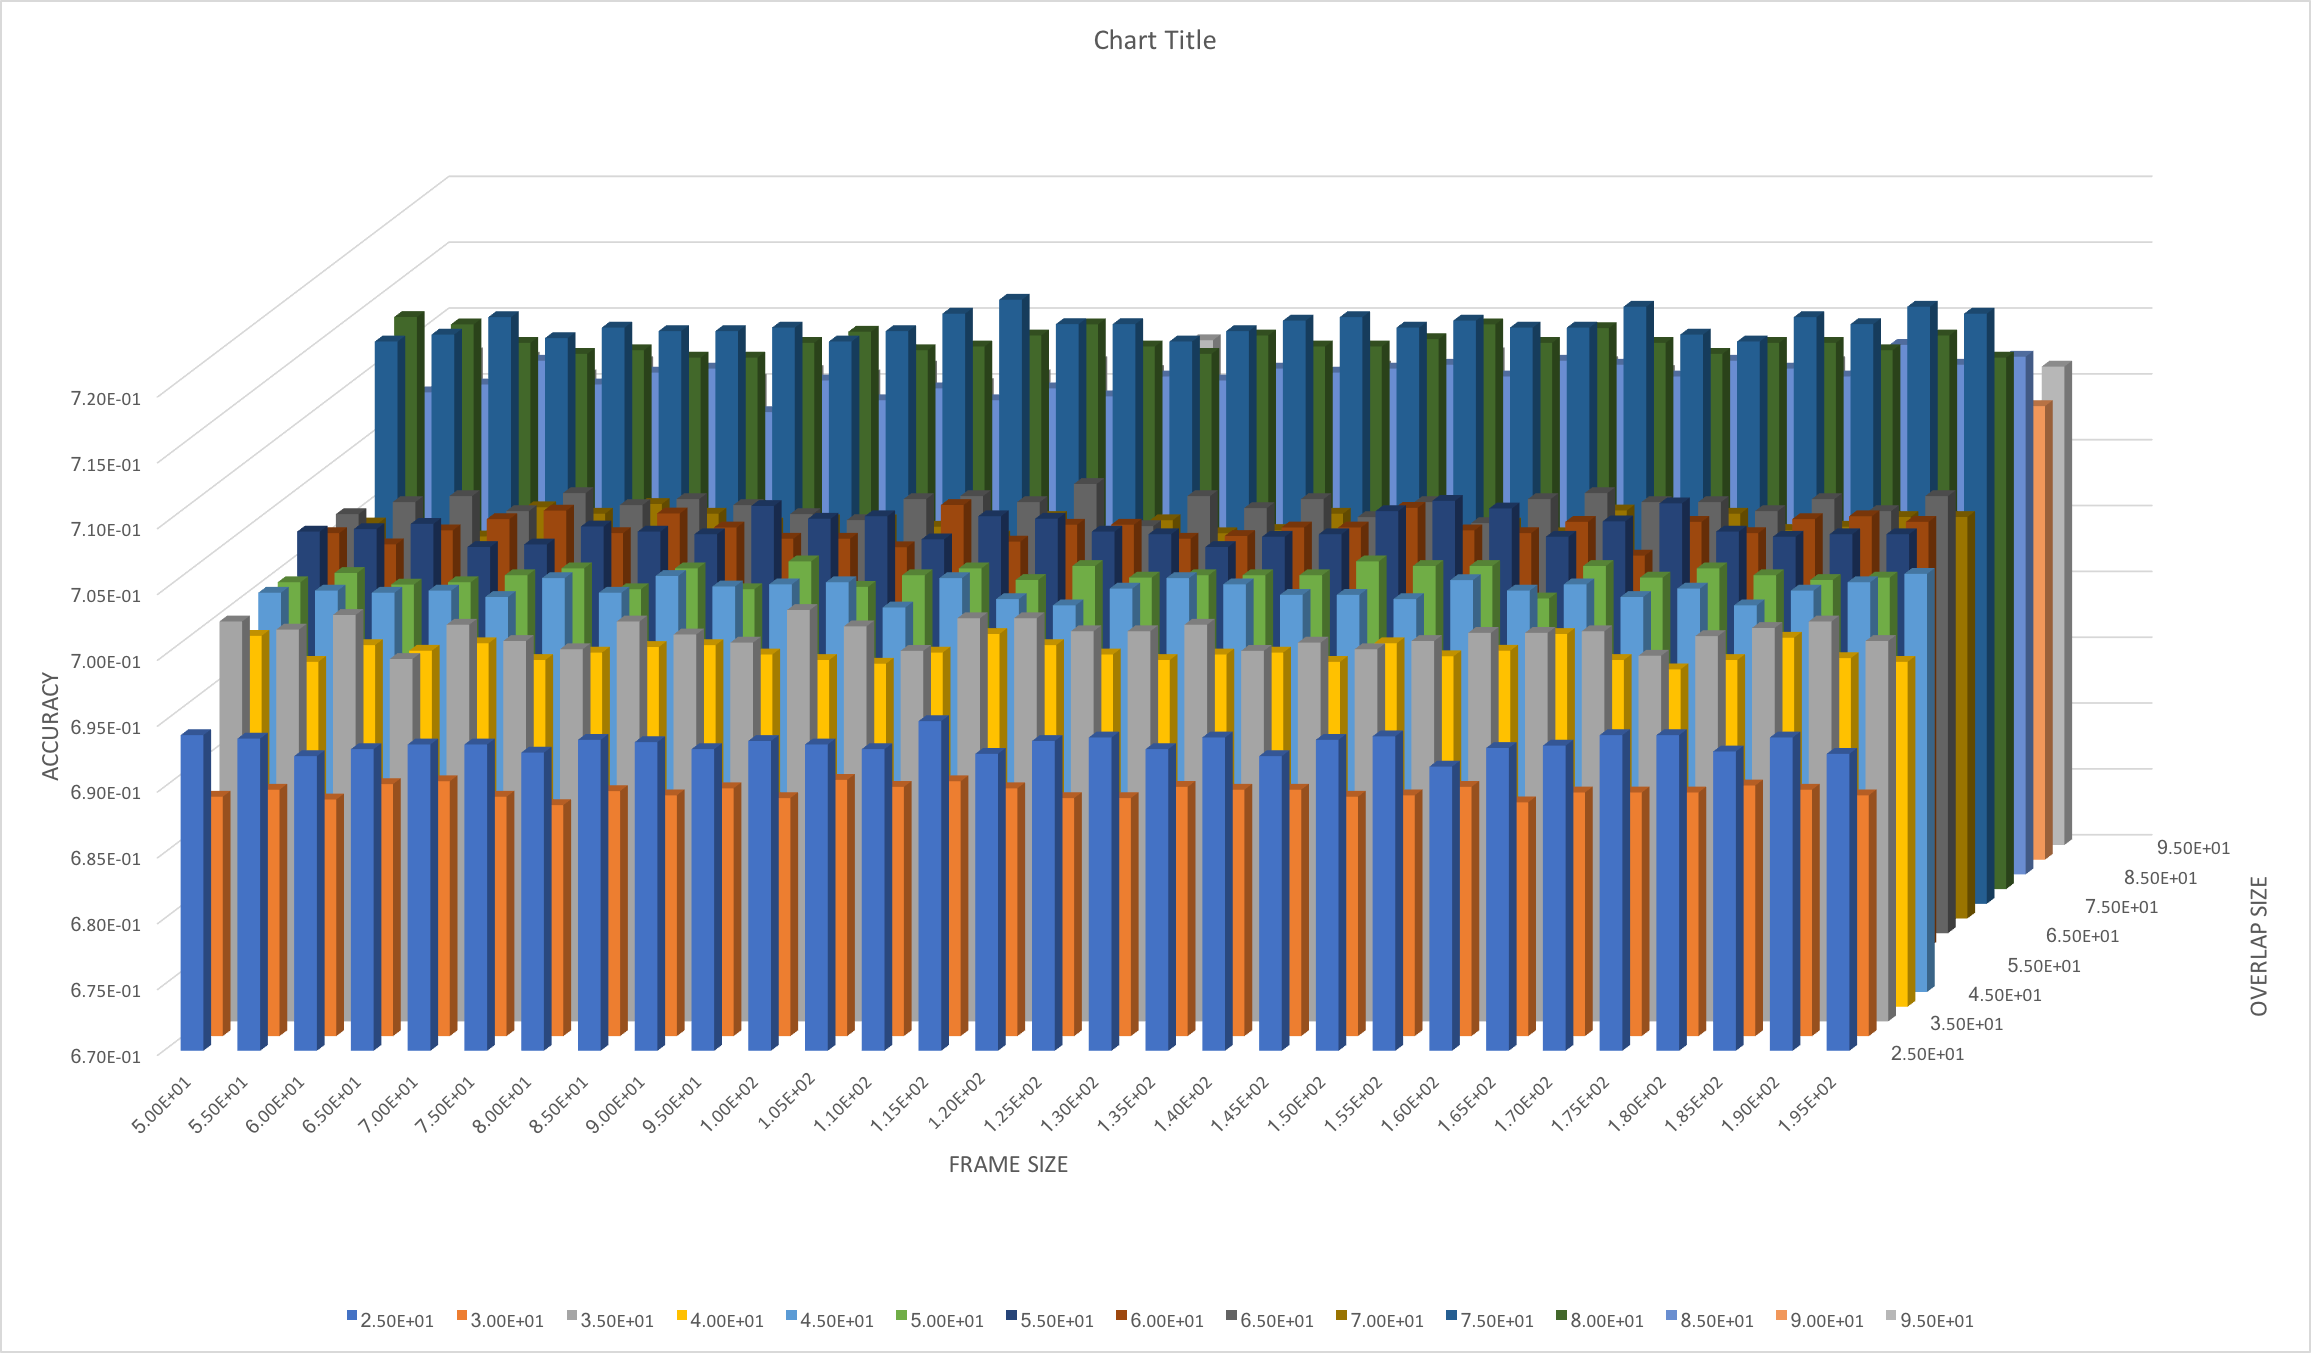
\includegraphics[scale=0.25]{PictureKNN.png}
\caption{Accuracy plot for KNN}
\label{fig:picKNN}
\end{figure*}

Since it was difficult to zero down on a fixed value of frame size and step size from this range,for each of the combination of frame size and step size, we extracted the features.
Next, the training data was separated from the test data using split train test technique. To select a test dataset from the available data, a random point was chosen within the dataset, and a block of data was extracted from this point. The size of the block was 1/10th of the total size of each dataset. This test data block was removed from the training data, thereby making sure that there is no overlap at all between training and testing data. The training data was then labeled and shuffled completely. Then it was trained and tested iteratively for different combinations of frame size and step size. Accuracy of both Random Forest and KNN classifier was recorded for each pair of frame size and step size. From a graph plotted between Accuracy, Frame Size and Step size for Random Forest (Fig\ref{fig:picRF}) and  KNN (Fig\ref{fig:picKNN} we found out the values of Frame Size and Step Size which gave us the maximum accuracy. \\
For choosing the correct classifier different classifiers were tried.


\begin{enumerate}
\item \textbf{SVM (RBF)}:Kernelized SVMs require the computation of a distance function between each point in the dataset, which is the dominating cost of (n features \textsc{\char42}  n\textsuperscript{2} observations). The storage of the distances is a burden on memory, so they\textsc{\char39}re recomputed on the fly. An accuracy of 58\textsc{\char37} was obtained, but the full simulation could not be completed due to computational intensity.
\item \textbf{KNN}:
N\textsc{\char95}neighbors: 4 (5 different classes of data)
With KNN an accuracy of 72.28\textsc{\char37} was obtained, for frame size of 105 and overlap of 75.

\item \textbf{Random Forest}:
n\textsc{\char95}estimators: 10 (trial and error)
An accuracy of 79.04\textsc{\char37} was obtained, for frame size of 90 and overlap of 80.
\end{enumerate}

\end{enumerate}


\section{Discussion}
Feature selection is an important criterion in activity recognition. Changing the classifier to obtain accuracy works upto certain threshold beyond which the accuracy becomes constant. But accuracy depends a lot on the feature vector used. The importance of each feature and the way they affected the accuracy of the classifier were studied and understood. 

\section{Future Work}
In this project, training of the model and conducting studies were performed with a limited number of locations and volunteers. The project can be extended for more locations with data collected by more volunteers to see how well it performs with increased number of locations with similar activities being performed. The accuracy of the classifier should go up with more data from different persons coming in but at the same time it is expected that addition of more locations will result in reduction of accuracy.
Currently, the wearable device which was used did not have a barometer sensor. If barometer sensor is included, it can be used to find out the exact floor in the building based on those readings. Also, these readings will improve the accuracy of the user location as different locations have different barometric readings\cite{Banerjee:2015:IFL:2802083.2802089}.

Magnetometer can be used to locate a user by employing the technique of magnetic finger-printing. Indoor location tend to have high magnetic field values because of objects like pillars and electrical-appliances\cite{Tachikawa:2016:PLS:2971648.2971684}\cite{Wang:2012:NNW:2307636.2307655}. Apart from this the magnetic sensor data varies a lot for outdoor and semi-outdoor places. The magnetic sensor data is also affected by the presence of people and in crowded environments shows a high fluctuation\cite{Zhang:2011:FSF:2318776.2318798} which can be further used to differentiate such places.

\section{Conclusion}
In this paper, an in-depth research study was presented, demonstrating how inertial sensing data can be an accurate location estimator for ubiquitous computing. Result of 79.04\textsc{\char37} accuracy using a random forest classifier was obtained. The confusion matrix for the KNN classifier (Table\ref{table:tableKNN}) and Random Forest (Table \ref{table:tableRF}) were plotted. From the results, it was analyzed that our classifier performs well even in cases where the activity done is similar but the location context is different. This is demonstrated by the ability of the classifier to distinguish stacking of books in library from shopping at a grocery store. Adding more data and locations as mentioned before, can improve the accuracy even further.

\bibliographystyle{abbrv}
\bibliography{sigproc}

%\balancecolumns 
\appendix
\section{Distribution of Work}
\subsection{Data Collection}
Gayatri Sivaraman, Jayant Bedwal, Shailesh Kelkar, Srihari Venugopalan
\subsection{Preprocessing}
Gayatri Sivaraman, Jayant Bedwal, Srihari Venugopalan
\subsection{Frame Extraction}
Gayatri Sivaraman
\subsection{Feature Extraction}
Jayant Bedwal, Srihari Venugopalan
\subsection{Training Model}
\subsubsection{Random Forest}
Shailesh Kelkar, Srihari Venugopalan
\subsubsection{KNN}
Shailesh Kelkar, Srihari Venugopalan
\subsubsection{SVM}
Gayatri Sivaraman, Jayant Bedwal
\subsubsection{Logistic Regression}
Gayatri Sivaraman, Jayant Bedwal
\subsection{Result Compilation and Analysis}
Gayatri Sivaraman, Jayant Bedwal, Shailesh Kelkar, Srihari Venugopalan
\end{document}
